\documentclass{article}

%----------------------------------------
% Packages
%----------------------------------------
\usepackage[left=1in, right=1in, top=1in, bottom=1in]{geometry}
\usepackage{graphicx}
\usepackage{amsmath,amsbsy,amssymb,amsfonts,amsthm}
\usepackage{nicefrac}
\usepackage{mathtools}
\usepackage{color}
\usepackage{xspace} % Correct macro spacing
\usepackage[numbers]{natbib} % For citations
\usepackage{times}
\usepackage{graphicx,subfigure}
%\usepackage[small,bf]{caption}
\usepackage{algorithm,algorithmic} 
\usepackage{hyperref}

\usepackage{shadethm}
\usepackage{fancyhdr}
\pagestyle{fancy}
\lhead{This is my name}
\rhead{this is page \thepage}
\usepackage[table,xcdraw]{xcolor}
\usepackage{pgfplots}
\usepackage{tabularx}
\usepackage{fancyhdr}
\pagestyle{fancy}
\lhead{IFT 6085 - Theoretical principles for deep learning}
\rhead{Lecture 3: January 15, 2020}


\newshadetheorem{thm}{Theorem}
\newshadetheorem{defn}[thm]{Definition}
\newshadetheorem{assm}[thm]{Assumption}
\newshadetheorem{prop}[thm]{Property}
\newshadetheorem{eg}[thm]{Example}
\newshadetheorem{lemma}[thm]{Lemma}


\usepackage{amsmath}

\DeclareMathOperator*{\argmax}{\arg\max}
\DeclareMathOperator*{\argmin}{\arg\min}
\DeclareMathOperator*{\E}{\mathbb{E}}
\DeclareMathOperator*{\I}{\mathbb{I}}
\DeclareMathOperator*{\V}{\mathbb{V}}

\newcommand{\diag}[0]{\operatorname{diag}}
\newcommand{\vect}[1]{\mathbf{#1}}
\newcommand{\vects}[1]{\boldsymbol{#1}}
\newcommand{\matr}[1]{\mathbf{#1}}
\newcommand{\matrs}[1]{\boldsymbol{#1}}

\renewcommand{\P}[0]{\mathbb{P}}
\newcommand{\Q}[0]{\mathbb{Q}}

\DeclareMathOperator*{\tr}{tr}
\DeclareMathOperator*{\prox}{prox}
\DeclareMathOperator*{\conv}{conv}
\DeclareMathOperator*{\dom}{dom}
\DeclareMathOperator*{\minimize}{minimize}
\DeclareMathOperator*{\maximize}{maximize}
\DeclareMathOperator*{\sign}{sign}
\DeclareMathOperator*{\vecop}{vec}
\DeclareMathOperator*{\Poisson}{Poisson}
\DeclareMathOperator*{\Cat}{Cat}
\DeclareMathOperator*{\Dir}{Dir}
\DeclareMathOperator*{\Exp}{Exp}
\DeclareMathOperator*{\DiscreteUniform}{DiscreteUniform}
\DeclareMathOperator*{\Uniform}{Uniform}
\newcommand{\R}{\mathbb{R}}
\newcommand{\N}{\mathbb{N}}
\newcommand{\X}{\mathcal{X}}

\DeclarePairedDelimiter{\abs}{\lvert}{\rvert}
\DeclarePairedDelimiter{\norm}{\lVert}{\rVert}
\DeclarePairedDelimiter{\inprod}{\langle}{\rangle}
\DeclarePairedDelimiter{\biginprod}{\big\langle}{\big\rangle}
\DeclarePairedDelimiter{\Biginprod}{\Big\langle}{\Big\rangle}
\DeclarePairedDelimiter{\bigginprod}{\bigg\langle}{\bigg\rangle}
\DeclarePairedDelimiter{\Bigginprod}{\Bigg\langle}{\Bigg\rangle}
\DeclarePairedDelimiter{\floor}{\lfloor}{\rfloor}

\definecolor{shadethmcolor}{HTML}{F0F0F0}
%\definecolor{shadethmcolor}{HTML}{EDEDED}
%\definecolor{shadethmcolor}{HTML}{EDF8FF}
%\definecolor{shaderulecolor}{HTML}{EDF8FF}
%\definecolor{shaderulecolor}{HTML}{45CFFF}
\setlength{\shadeboxrule}{.4pt}

\setlength\parindent{0pt}

% Packages hyperref and algorithmic misbehave sometimes.  We can fix
% this with the following command.
\newcommand{\theHalgorithm}{\arabic{algorithm}}

%----------------------------------------
% Standard macros
%----------------------------------------


%----------------------------------------
% Project-specific macros
%----------------------------------------

%----------------------------------------
% Header
%----------------------------------------
\title{IFT 6085 - Lecture 3 \\ 
Gradients for smooth and for strongly convex functions}
\date{}
%----------------------------------------
% Document
%----------------------------------------
\begin{document} 

%----------------------------------------
% Abstract
%----------------------------------------
\maketitle

\vspace{-0.5in}
\begin{center}
This version of the notes has not yet been thoroughly checked.
Please report any bugs to the scribes or instructor.
\end{center}
\vspace{0.2in}

\textbf{Scribes}\hfill
\textbf{Instructor:}  Ioannis Mitliagkas\\
\textbf{Winter 2020:} Thong (Bob) Vo\\
\textbf{Winter 2019:} Amir Raza, Philippe Lacaille, Jonathan Plante\\
\textbf{Winter 2018:} Philippe Brouillard, Massimo and Lucas Caccia


%----------------------------------------
% Body
%----------------------------------------

\newcommand{\infgc}{\inf_{g \in \mathcal{C}}}
\newcommand{\supgc}{\sup_{g \in \mathcal{C}}}

\newcommand{\Prob}{\mathbb{P}}
\newcommand{\reals}{\mathbb{R}}

\section{Summary}

In the previous lecture we covered the notions of convexity as well as Lipschitsz continuity. After introducing these concepts, a bound on the convergence rate of gradient descent of a convex and $L$-Lipschitz function was demonstrated to scale with the $\sqrt{T}$.
\\

Building on some of the previous lecture notions, we will introduce guarantees on the convergence rate of gradient descent for a stronger family of functions (using stronger assumptions), namely $\beta$-smooth and $\alpha$-strong convex functions.
\\

\section{Gradient Descent for smooth functions}

\begin{defn}[$\beta$-smoothness]
We say that a continuously differentiable function $f$ is $\beta$-smooth if its gradient $\nabla f$ is $\beta$-Lipschitz, that is 
\[
	\| \nabla f(x) - \nabla f(y)\| \leq \beta \| x-y \|
\]
\end{defn}
If we recall Lipschitz continuity from Lecture 2, simply speaking, an \textit{L-}Lipschitz function is limited by how \textit{quickly} its output can change. By imposing this same constraint on the gradients of a function, $\beta$-smoothness implies they cannot change abruptly and must be bounded by some value as defined above.
\\

% \begin{figure}[ht]
% \centering
%     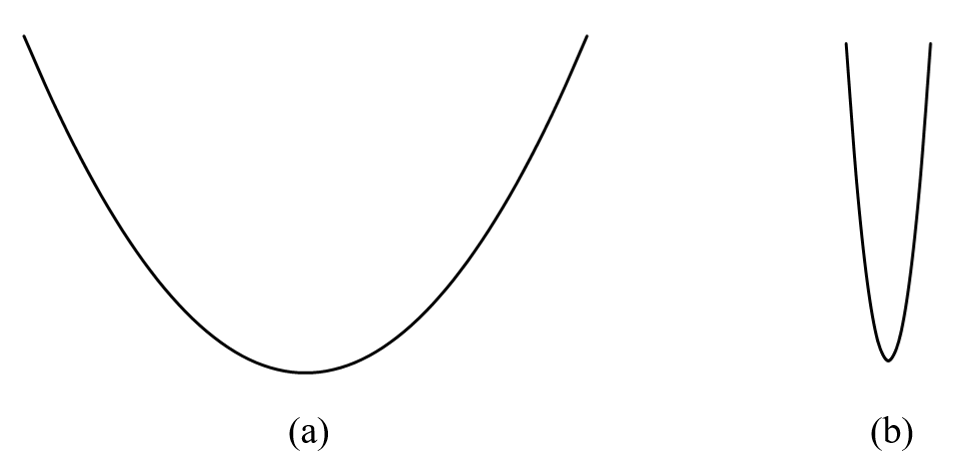
\includegraphics[width=0.58\textwidth]{BSmoothPic.png}%
%     \caption{(a) A $\beta$-smooth function. (b) A non $\beta$-smooth function}
%     \label{str_convex}
% \end{figure}

In other other words, $\beta$-smoothness is putting an upper bound on the curvature of the function. This is equivalent to the eigenvalues of the Hessian being less than $\beta$. Note that there can be $\beta$-smooth functions which are not twice differentiable. One key benefit of these functions is that their gradients tend to decay when $x$ gets closer to the minimum. In contrast, non-smooth functions may have abrupt bends at the minimum, which cause significant oscillations for gradient descent. Figure \ref{fig:gradient_updates} illustrates this point by comparing the two scenarios.
\begin{figure}[ht]
\centering
    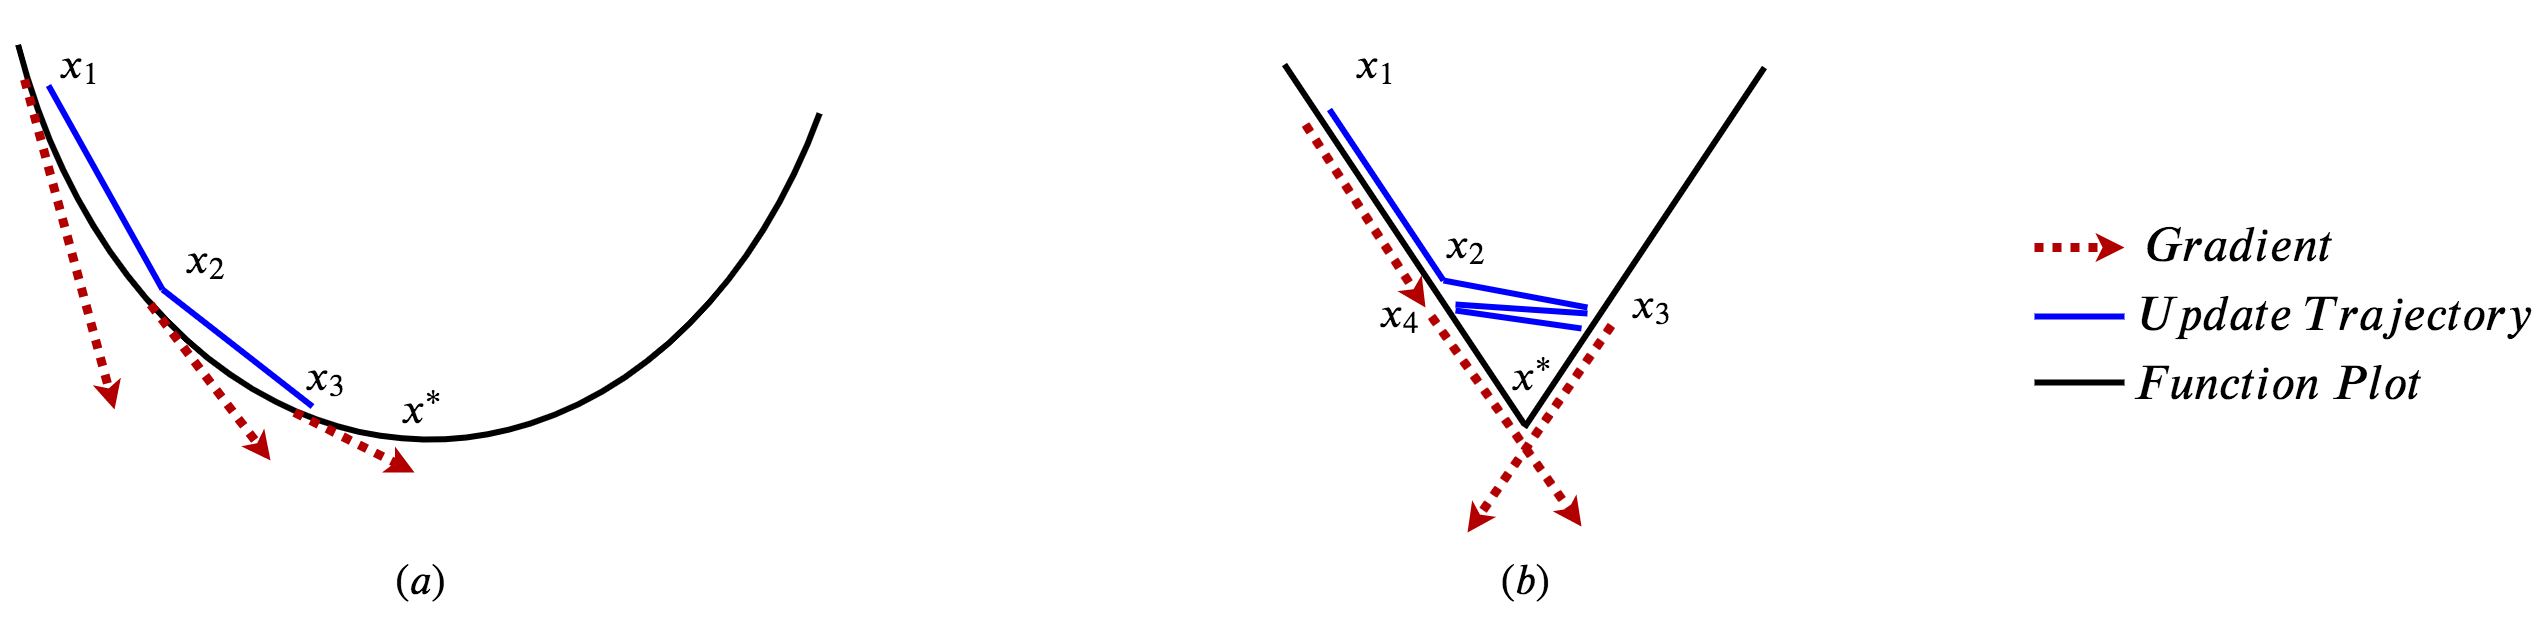
\includegraphics[width=0.87\textwidth]{gradient_swing_legends.png}%
    \caption{(a) A smooth function with decaying updates. (b) A non-smooth function with oscillating updates.}
    \label{fig:gradient_updates}
\end{figure}


\subsection{Convex and smooth functions}

Here we introduce a bound on the convergence rate of a convex and $\beta$-smooth function.

\begin{lemma}[Quadratic bounds]\label{lemma:smooth-sandwich}
	Let $f$ be $\beta$-smooth on $\mathbb{R}^n$. Then for any $x,y$ $\in \mathbb{R}^n$, one has
     \begin{equation} \label{eq:lemma34}
	|f(x) - f(y) - \nabla f(y)^\intercal (x-y) | \leq \dfrac{\beta}{2} \| x-y \|^2
    \end{equation}
%See \cite{bubeck2015convex} Lemma 3.4 for proof.
\end{lemma}

\begin{proof} Let $g: \mathbb{R}\to \mathbb{R}$ by the rule $g(t) \triangleq f(y+t(x-y))$. The following holds true:
$$f(x)=g(1) \: and \: f(y) = g(0)$$

Then, we also observe that:
\begin{equation} \label{eq:gtintegral}
f(x) - f(y) = g(1) - g(0) = \int_{0}^{1}g'(t) \, dt 
\end{equation}
Taking derivative of $g(t):$

\begin{equation} \label{eq:gtderivative}
g'(t) = \nabla f(y+t(x-y))^T (x-y)
\end{equation}

Plugging in Equation \ref{eq:gtintegral}, and \ref{eq:gtderivative} to the LHS of \ref{eq:lemma34}:

\begin{align*}
	&	|f(x) - f(y) - \nabla f(y)^\intercal (x-y) |&\\
	&= |\int_{0}^{1} \nabla f(y+t(x-y))^\intercal (x-y) \, dt - \nabla f(y)^\intercal (x-y) |\\
	&\leq \int_{0}^{1} |\nabla f(y+t(x-y)-\nabla f(y))^\intercal (x-y)|\, dt\\
	&\leq \int_{0}^{1} \|\nabla f(y+t(x-y))-\nabla f(y)\| \cdot \|x-y \|  \, dt \tag{applying Cauchy–Schwarz inequality  } \\
	&\leq \int_{0}^{1} \beta t|x-y \|^2  \, dt \tag{the gradient $\nabla f$ is $\beta$  -Lipschitz.} \\
	&= \frac{\beta}{2}\|x-y\|^2 \,
\end{align*}{}


\end{proof}


\begin{lemma}
	Let $f$ be such that $0 \leq f(x)-f(y)-\nabla f(y)^\intercal(x-y) \leq \dfrac{\beta}{2} \| x-y \|^2$. Then for any $x,y$ $\in \mathbb{R}^n$, one has
 \[
	f(x) - f(y) \leq \nabla f(x)^\intercal (x-y) - \dfrac{1}{2 \beta} \| \nabla f(x)-\nabla f(y) \|^2
\]    
\end{lemma}
\begin{proof}
\textit{See \cite{bubeck2015convex} Lemma 3.5 for proof.}
\end{proof}


\begin{thm}\label{thm:cvx-smth}
Let $f$ be convex and $\beta$-smooth on $\mathbb{R}^n$. Then the gradient descent with step size $\gamma = 1/\beta$ satisfies
\[
	f(x_{k}) - f(x^{*}) \leq \dfrac{2 \beta \| x_1 - x^{*} \|^2}{k-1}
\]
\end{thm}

\begin{proof}
\textit{See \cite{bubeck2015convex} page 268.}
\end{proof}


In comparison to the convergence analysis for a convex and \textit{L-}Lipschitz function, the following points of improvement are observed in Theorem \ref{thm:cvx-smth} over the previous result:

\begin{itemize}
\item No averaging of terms 
\item $x_{k}$  is a good solution, i.e. no reference to previous iterations
\item Convergence scales linearly with number of steps, convergence rate of order $O(1/T)$ compared to $O(1/\sqrt{T})$
\item Ideal step size $\gamma$ is constant and does not depend on T (number of steps taken).
\end{itemize}
As an observation of ${\| x_1 - x^{*} \|^2}$, the bound will be tighter if $x_1$ will be closer to $x^{*}$ (minima), and looser if $x_1$ will be farther. Bounds that don't depend on the initial value of $x$ will be discussed later in this lecture.

\section{Strong convexity}

\begin{defn}[Strong convexity]
A function $f(x)$ is $\alpha$-strongly convex, if for $\alpha>0$, $\forall x\in\dom(f)$, 
\begin{align*}
f(x) - \frac{\alpha}{2} \norm{x}^2 \text{is convex.}
\end{align*}
\end{defn}

Strong convexity provides a lower bound for the function's curvature. The function must have strictly positive curvature. In other words, all eigenvalues of the Hessian of a $\alpha$-strongly convex function are lower bounded by $\alpha$. We can write this in terms of positive-semi definiteness as
\[
\nabla^2 f(x) \succeq \alpha I  \iff  \nabla^2 f(x) - \alpha I \succeq 0
\]

For example, $f:\R\to\R, f(x) = \frac{h}{2} x^2$ is $h$-strongly convex, but not $(h+\epsilon)$-strongly convex for $\epsilon>0$. Figure~\ref{str_convex} illustrates examples of two convex functions, of which only one is strongly convex.\\

\begin{figure}[ht]
\centering
    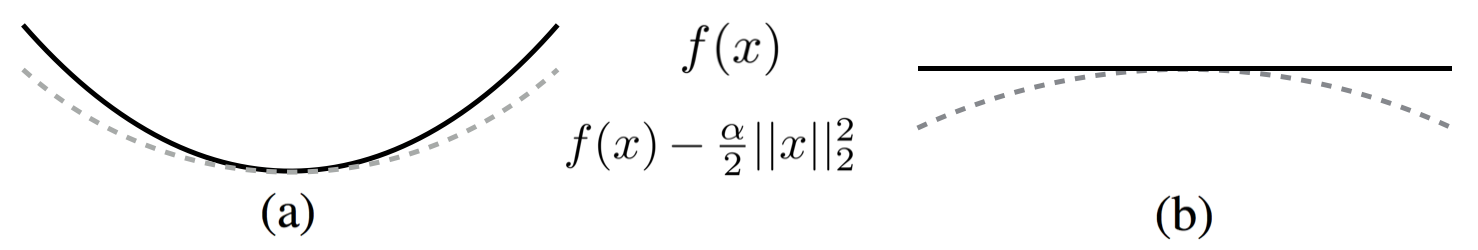
\includegraphics[width=0.58\textwidth]{str_convex.png}%
    \caption{(a) A convex function which is also strongly convex. (b) A convex function which is not strongly convex.}
    \label{str_convex}
\end{figure}




\subsection{Strongly convex and Lipschitz functions}
\begin{thm}\label{thm:str-cvx-lipschitz}
	Let $f$ be $\alpha$-strongly convex and $L$-Lipschitz. Then the projected subgradient descent after $T$ steps with $\gamma_k = \dfrac{2}{\alpha(k+1)}$ satisfies  
\[
	f\left(\sum_{k=1}^T \dfrac{2k}{T(T+1)} x_k \right) - f(x^{*}) \leq \frac{2 L^2}{\alpha(T+1)}
\]
\end{thm}

\begin{proof}
\textit{See \cite{bubeck2015convex} page 277}
%%%%%%%%%%%%%
% to do
%%%%%%%%%%%%%
\end{proof}

With Theorem \ref{thm:str-cvx-lipschitz}, we can notice how moving from convexity to strong convexity may affect the convergence rate of gradient descent. We previously tackled convexity paired with Lipschitz continuity in Lecture 2 and the similarity with the new convergence guarantees is pretty noticeable. By moving to strong-convexity, we can notice a few things:
\begin{itemize}
    \item Still have averaging of terms, where $\sum\limits_{k=1}^T \dfrac{2k}{T(T+1)} x_k$ is a non uniform averaging scheme with more recent iterates having more weight
    \item Current $x_k$ solution is not appropriate, i.e. ideally only evaluate at $x_k$
    \item Convergence now scales linearly with number of steps
    \item Although not constant, the step size $\gamma_k$ is diminishing at every step
\end{itemize}

\vspace{3mm}
Unlike previous results, the right hand side does not have any terms dependent on distance from $x^{*}$ here. Intuitively this is a consequence of two conditions which have to be met for a Strong Convex function:
\begin{itemize}
    \item Norm of Gradient increases as we go further away from minima.
    \item Gradient for a L-Lipschitz function is bounded, and can not keep increasing.
\end{itemize}
Thus to have a finite bound, no distance term on the right hand side of the bound.
\vspace{3mm}

One could hope that by combining strong convexity along with smoothness, gradient descent may present stronger convergence guarantees. We will see how smoothness removes dependency from the averaging scheme.

\vspace{3mm}
Note: $\alpha $ Strongly convex and L-Lipschitz condition is a special case because the upper bound L-Lipschitz condition will ultimately conflict with the lower bound $\alpha $ Strongly convex grow rate. Therefore, such functions are typically defined in a range, e.g. $x \in [-1,1]$.

\subsection{Strongly convex and smooth functions}

Recalling Lemma \ref{lemma:smooth-sandwich} (Quadratic bounds), it tells us that a $\beta$-smooth function $f$ is sandwiched between 2 quadratics because of the following inequality:

\begin{align}\label{eq:smooth-bound}
f(y) + \nabla f(y)^\intercal (x-y) - \dfrac{\beta}{2} \| x-y\|^2 \leq f(x) \leq f(y) + \nabla f(y)^\intercal (x-y) + \dfrac{\beta}{2} \| x-y\|^2
\end{align}
 


Now we introduce another lemma which allows us to lower bound an $\alpha$-strong convex function.

\begin{lemma}\label{lemma:str-cvx-bound}
Let $f$ be $\lambda$-strongly convex. Then $\forall x, y$, we have:
\begin{align*}
f(y) - f(x) \leq \nabla f(y)^T(y-x) - \frac{\lambda}{2} \norm{x - y}^2
\end{align*}
The strong convexity parameter $\lambda$ is a measure of the curvature of $f$.
\end{lemma}

By rearranging terms, this tells us that a $\lambda$-strong convex function can be lower bounded by the following inequality:

\begin{align}\label{eq:str-cvx-bound}
f(x) \geq f(y) - \nabla f(y)^T(y-x) + \frac{\lambda}{2} \norm{x - y}^2
\end{align}

Figure \ref{fig:bounds} showcases the resulting bounds from both the smoothness and the strong convexity constraints. The shaded area in each sub-figure is showing the area validated by the respective bound(s).

\begin{figure}[ht]
    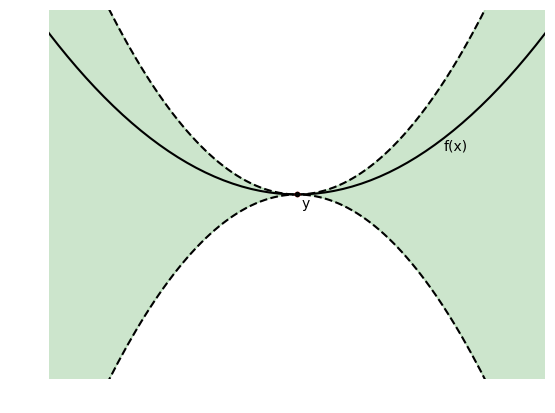
\includegraphics[width=.32\textwidth]{smooth-bound.png}\hfill
    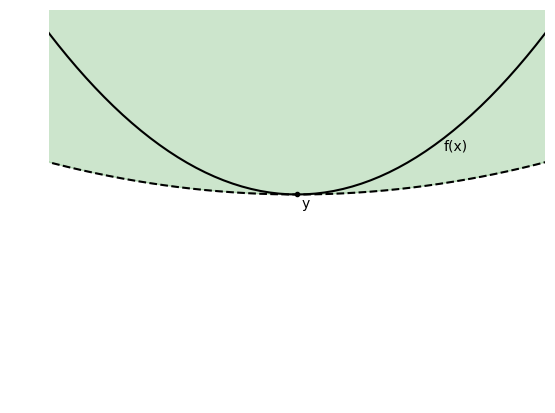
\includegraphics[width=.32\textwidth]{str-cvx-bound.png}\hfill
    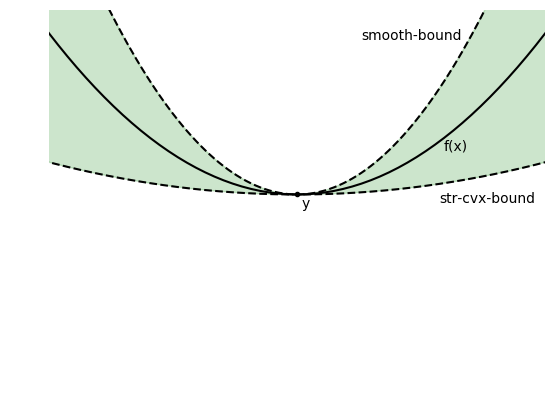
\includegraphics[width=.32\textwidth]{smooth-str-cvx-bound.png}

    \caption{(Left) Upper and lower bounds from equation \ref{eq:smooth-bound} for smoothness constraint (Middle) Lower bound from equation \ref{eq:str-cvx-bound} for strong convexity constraint (Right) Combination of upper bound from smoothness and lower bound from strong convexity}
    \label{fig:bounds}
\end{figure}

\begin{figure}[h]
\centering
    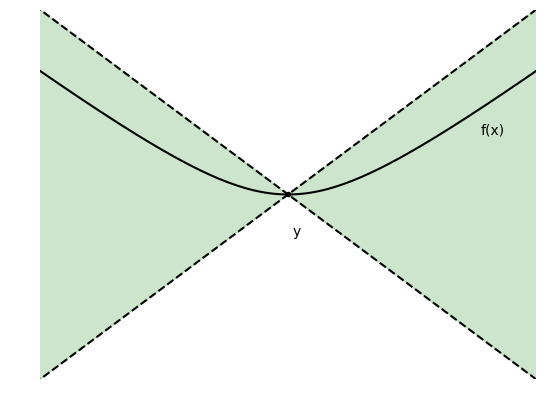
\includegraphics[width=0.4\textwidth]{lipschitz-bound.png}
    \caption{For an $L_f$-Lipschitz continuous function, the green region shows where the function would exist . We can imagine that without smoothness and only L-Lipschitz in equation \ref{eq:smooth-bound}, the accepted region would be having linear boundaries}
    \label{fig:accepted-reg}
\end{figure}


\begin{lemma}[Coercivity of the gradient] Let $f$ be $\beta$-smooth and $\lambda$-strongly convex. Then for all $x$ and $y$, we have:
$$ \langle \nabla f(x) - \nabla f(y), x-y \rangle \geq \frac{\lambda\beta}{\lambda + \beta} \| x-y\|^2 + \frac{1}{\lambda + \beta} \| \nabla f(x) - \nabla f(y) \|^2 $$

\end{lemma}

\begin{proof}
\textit{See \cite{bubeck2015convex} Lemma 3.11 for proof.}
\end{proof}
\begin{thm}\label{thm:str-cvx-smth}
For $f$ a $\lambda$-strongly convex and $\beta$-smooth function, gradient descent with $\gamma = \frac{2}{\lambda + \beta}$ satisfies:
\[
	f(x_{k+1}) - f(x^{*}) \leq \frac{\beta}{2} \exp \left( -\frac{4k}{\kappa + 1} \right) \| x_1 - x^{*} \|^2
\]
where $\kappa \triangleq \frac{\beta}{\lambda}$ is the condition number.
\end{thm}

\begin{proof} (Theorem \ref{thm:str-cvx-smth}) First, let's define the distance between the coordinate at the iteration $k$ and the optimal point as:
$$ D_k \triangleq \| x_k - x^{*}\|$$
Then,
$$ D_{k+1}^2 = \| x_{k+1} - x^{*} \|^{2} $$

By replacing $x_{k+1}$ by its definition $x_k - \gamma \nabla f(x_k)$, we get:
$$ D_{k+1}^2 = \| x_k - \gamma \nabla f(x_k) - x^{*} \|^{2} $$

By expanding the square, we get:
$$ D_{k+1}^2 = \| x_k - x^{*} \|^2 - 2 \gamma \langle \nabla f(x_k), x_k - x^{*} \rangle + \gamma^2 \| \nabla f(x_k) \|^2 $$

By doing a slight modification to the second term, we can apply the lemma of coercivity of the gradient. Since $ \nabla f(x^{*}) = 0$ this equality holds:
$$ \langle \nabla f(x_k), x_k - x^{*} \rangle = \langle \nabla f(x_k) - \nabla f(x^{*}), x_k - x^{*} \rangle $$
And by applying the lemma of coercivity of the gradient, we get an upper bound:
$$ \langle \nabla f(x_k) - \nabla f(x^{*}), x_k - x^{*} \rangle \geq \frac{\lambda \beta}{\lambda + \beta} D^2_k + \frac{1}{\lambda + \beta} \| \nabla f(x_k) - \nabla f(x^{*}) \|^2 $$

By replacing the second term by the upper bound we just found, we get:
$$ D^2_{k+1} \leq D^2_k - 2 \gamma \left(\frac{\lambda \beta}{\lambda + \beta} D^2_k + \frac{1}{\lambda + \beta} \| \nabla f(x_k)\|^2\right) + \gamma^2 \| \nabla f(x_k) \|^2$$
We can rearrange the terms and add $ - \nabla f(x^{*})$ again inside the norm terms:
$$ D_{k+1}^2 \leq \left(1 - \frac{2\gamma \lambda \beta}{\lambda + \beta}\right) D^2_k + \left( \frac{-2\gamma}{\lambda + \beta} + \gamma^2 \right) \| \nabla f(x_k) - \nabla f(x^{*}) \|^2$$

The term $\left(1-\frac{2\gamma \lambda \beta}{\lambda + \beta}\right)$ is useful, because we can show that it is less than 1 and has geometric convergence. Further steps will try to simplify the remaining terms.

We can change the norm term by using the fact that $f$ is $\beta$-smooth:
$$ D_{k+1}^2 \leq \left( 1 - \frac{2\gamma \lambda \beta}{\lambda + \beta}\right)  D^2_k + \left( \frac{-2\gamma}{\lambda + \beta} + \gamma^2 \right) \beta^2 D^2_k $$

Let $ \gamma = \frac{2}{\lambda + \beta} $, then:
$$ D^2_{k+1} \leq \left( 1 - \frac{4 \lambda \beta}{(\lambda + \beta)^2} \right) D^2_k $$

By unrolling the recursion and since $ \left( \frac{\kappa - 1}{\kappa + 1} \right)^2 = \left( 1 - \frac{4 \lambda \beta}{(\lambda + \beta)^2} \right) $ we get:
$$ D^2_{k+1} \leq \left( \frac{\kappa - 1}{\kappa + 1} \right)^{2k} D_1^2 $$

Since $\exp(-x) \geq 1-x$ for every $x$, we get:
$$ D_{k+1}^2 \leq \exp{\left( -\frac{4k}{\kappa + 1} \right)} D_1^2  $$

By $ \beta $-smoothness we finally have:

$$ f(x_{k+1}) - f(x^{*}) \leq \frac{\beta}{2} \exp{\left( -\frac{4k}{\kappa + 1} \right)} \| x_1 - x^{*} \|^2 $$

\end{proof}

Theorem \ref{thm:str-cvx-smth} observations
\begin{itemize}
    \item $x_k$ solution is a good solution, i.e. no reference to previous iterations
    \item Convergence rate of order $O(\exp(-T))$
    \item $\kappa$ measures how \textit{far apart} the upper and lower bounds are (see Figure \ref{fig:bounds}). It can be interpreted as the ratio of largest to smallest curvature of the function.
    \item The smaller the condition number $\kappa$ is, the less iterations are required to converge. Intuitively, the accepted region between the bounds will be smaller.
    \item Consequently, the greater $\beta$ is the more iterations will be required to converge. This is logical since a constant step size on a function with a steep gradient will cause the a greater change in the function value.
\end{itemize}
\pagebreak

\section{Comparison of optimization properties for different function classes }
The table below summarizes various convergence properties of discussed functions classes.  From left to right, the assumptions on properties of these classes increase, from Convex and L-Lipschitz to $\lambda$ strongly convex and $\beta$ smooth. In the same direction, the convergence rates are also increase, aligned with stronger assumptions on those functions.

\begin{table}[h]
\footnotesize
%\small
\renewcommand{\arraystretch}{1.8}
\centering
    \caption{Comparison of different function classes}
    \begin{tabularx}{\columnwidth}{|>{\hsize=0.8\hsize\linewidth=\hsize}X|>{\hsize=1.1\hsize\linewidth=\hsize}X|>{\hsize=0.8\hsize\linewidth=\hsize}X|>{\hsize=1.3\hsize\linewidth=\hsize}X|>{\hsize=1\hsize\linewidth=\hsize}X|}
        \hline
        Function Class & cvx, L-Lipschitz & cvx, $\beta$ smooth & $\alpha$ str-cvx, L-Lipschitz & $\lambda$ str-cvx, $\beta$ smooth \\
        \hline
        Optimal Step size & $\gamma = \frac{\norm{x_1 - x^\ast}_2}{L \sqrt{T}}$ & $\gamma = \frac{1}{\beta}$ & $\gamma = \frac{2}{\alpha (k+1)}$ & $\gamma = \frac{2}{\lambda + \beta}$ \\
        Convergence Rate     & $\mathcal{O}(1/\sqrt{T})$ & $\mathcal{O}(1/{T})$ &$\mathcal{O}(1/{T})$ & $\mathcal{O}(exp(-T))$    \\
        Sub-optimal gap       & $
f\left(\frac{1}{T}\sum_{k=1}^T x_k\right)-f(x^*)$ & $(x_{k}) - f(x^{*})$ & {\tiny $f\left(\sum_{k=1}^T \dfrac{2k}{T(T+1)} x_k \right)-f(x^{*})$ }& $f(x_{k+1}) - f(x^{*})$  \\
        Bounds of the gap & $\leq \frac{\norm{x_1 - x^\ast}L}{\sqrt{T}}$ & $\leq \dfrac{2 \beta \| x_1 - x^{*} \|^2}{k-1}$ & $ \leq \frac{2 L^2}{\alpha(T+1)} $ &  $\leq \frac{\beta}{2} \exp \left( -\frac{4k}{\kappa + 1} \right) D_1^2$ \\

        \hline
    \end{tabularx}
    \label{table: simulation parameters}
\end{table}
%----------------------------------------
% \section*{Acknowledgments} 

%----------------------------------------
\bibliographystyle{abbrvnat}
\bibliography{Refs/lec3}
%----------------------------------------
\end{document}
